\documentclass{article} % JASA requires 12 pt font for manuscripts
%\usepackage{JASA_manu}        % For JASA manuscript formatting

\usepackage{endfloat} % just for while I am writing

% for citations
\usepackage[authoryear]{natbib} % natbib required for JASA
\usepackage[dvips,colorlinks=true, citecolor=blue, linkcolor=blue]{hyperref}

%\definecolor{Blue}{rgb}{0,0,0.5}
\newcommand{\hh}[1]{{\color{orange} #1}}
\newcommand{\al}[1]{{\color{red} #1}}

% fonts
%\usepackage{kpfonts}

% for figures
\usepackage{graphicx}
\DeclareGraphicsExtensions{.eps, .pdf}
\graphicspath{{figures/}}

% help with editing and coauthoring
\usepackage{todonotes}

% title formatting
\usepackage[compact,small]{titlesec}

% page formatting
\usepackage[margin = 1in]{geometry}
\usepackage[parfill]{parskip}

% line spacing
\usepackage{setspace}
\doublespace

% For math typsetting
\usepackage{bm}
\usepackage{amstext}
\usepackage{amssymb}
\usepackage{amsmath}
\usepackage{amsfonts}
\usepackage{multirow}

% A few commands to make typing less tedious
\newcommand{\inv}{\ensuremath{^{-1}}}
\newcommand{\ginv}{\ensuremath{^{-}}}
\newcommand{\trans}{\ensuremath{^\prime}}
\newcommand{\E}{\ensuremath{\mathrm{E}}}
\newcommand{\var}{\ensuremath{\mathrm{Var}}}
\newcommand{\cov}{\ensuremath{\mathrm{Cov}}}


\title{Simulation-Based Diagnostics for Hierarchical Linear Models: A Graphical Approach}

\author{Adam Loy, Lendie Follett, Heike Hofmann, Dianne Cook\\
	Department of Statistics\\
	Iowa State University\\
	Ames, IA 50011-1210
}

\begin{document}
\maketitle
\begin{abstract}
Motivation for this paper: describe visual inference, and apply to (open) problems of diagnosing HLMs. Show a case study of an experiment for Q-Q plots. 
\end{abstract}

\tableofcontents
%------------------------------------------------------------------------------------
\section{Introduction}
%------------------------------------------------------------------------------------

Hierarchical linear models (i.e., multilevel models, linear mixed effects models, random coefficient models) are versatile models that allow for dependence expected when data are organized in hierarchical structures---such data structures are especially common in social science research where studies often focus on responses from human subjects. Examples of these structures include when subjects are naturally grouped by organization (e.g., student within schools), geography (e.g., voters within states), and interviewer (e.g., respondents assigned to an interviewer). The additional flexibility offered by these models to incorporate data from each level of the data hierarchy and allow for dependencies between individuals within the same group complicates model exploration and verification. More specifically, residual plots often display noticeable patterns, but these patterns are often artifacts of model estimation rather than indications of lack of fit. To mitigate the risk of detecting such artifacts we suggest a graphical simulation-based approach to model checking that makes use of the protocols from visual inference \citep{Buja:2009hp}.


%%------------------------------------------------------------------------------------
%\section{Visual inference}\label{sec:vi}
%%------------------------------------------------------------------------------------
In order to develop graphical model diagnostics as substitutes for statistical tests of model assumptions, we work within a rigorous inferential framework. \cite{Gelman:2004gg} formulates a visual analog of simulation-based model diagnostics in which a visualization of an aspect of the model is compared to data generated under the model. \cite{Buja:2009hp} extend this idea, proposing two protocols that formalize a rigorous inferential framework for testing visual discoveries. In this section we outline the lineup protocol.

Classical statistical inference consists of 
\begin{enumerate}
	\item formulating a null and alternative hypothesis,
	\item calculating a test statistic,
	\item comparing the test statistic to a reference (null) distribution,
	\item and calculating a $p$-value from on which we base our conclusion.
\end{enumerate}
Each of these steps has a direct analog in visual inference \citep{Buja:2009hp}. As we will apply visual inference for model diagnostics, we want to highlight these parallels in this framework: the null  hypothesis corresponds to some assumption about the model, such as e.g.~homogeneity of residual variance,
while
the alternative hypothesis encompasses any violation of this model assumption. For visual inference, the test statistic corresponds to a plot  that displays the model assumption and allows the observer to distinguish between scenarios under null and alternate hypothesis. 
A plot of data generated consistently with the null hypothesis is called a null plot. The set of all null plots makes the reference distribution. 
If the model assumption holds, i.e.  under the null hypothesis, the plot of the observed data is indistinguishable from the null plots. 
In the lineup protocol the true plot is randomly embedded among a number of null plots.  
\hh{Figure~\ref{fig:fanned} gives a first example of a lineup. Each panel shows  line segments of different lengths  with varying slopes. 
Observers are asked to identify the plot that is the most different from the other plots.    Any additional information is  withheld on purpose to prevent observers from (subconsciously)  introducing preconceived notions and making decisions that are not purely based on the data display. 
}
\begin{figure}
	\centering
	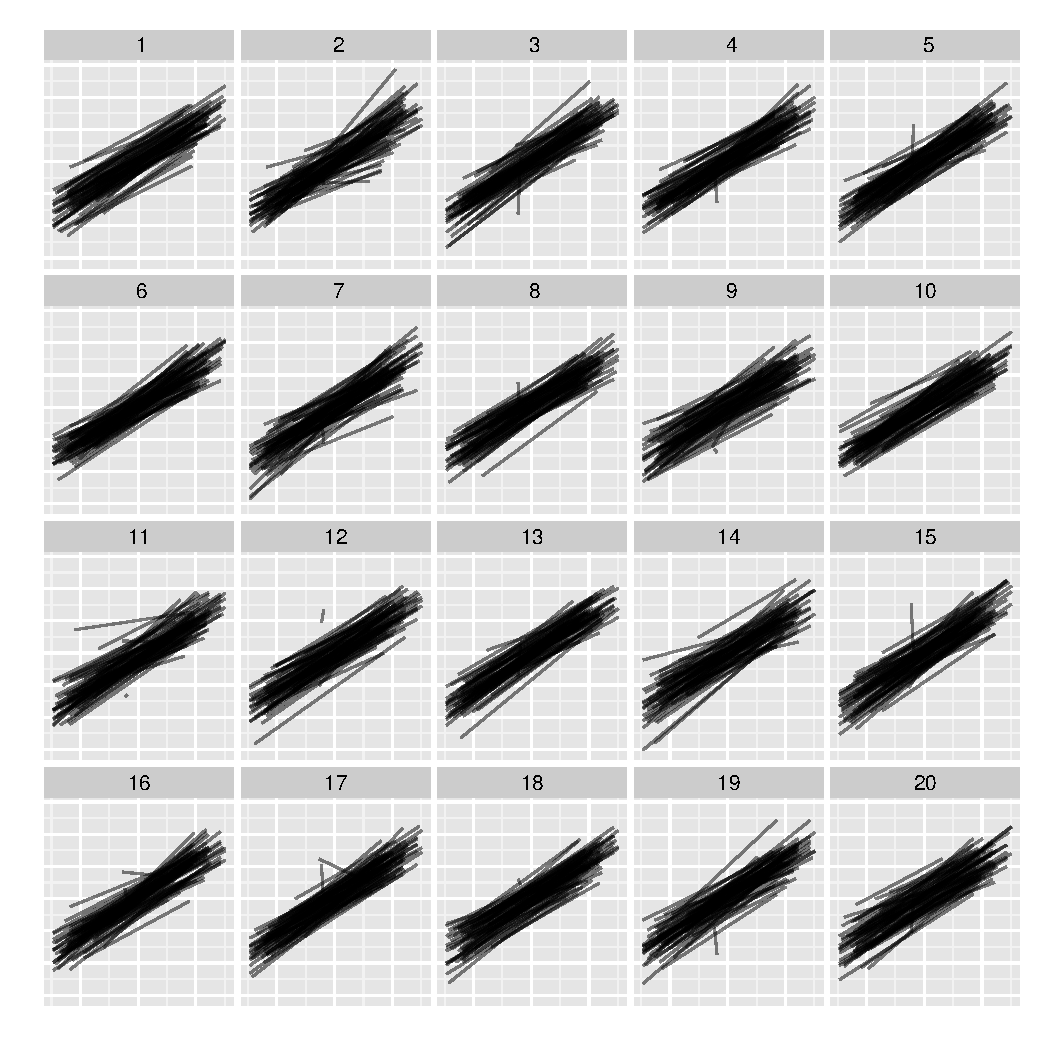
\includegraphics[width=\textwidth]{normexam_fanned_lineup13.pdf}
	\caption{\label{fig:fanned} \hh{Which plot is the most different from the other plots?} \hh{What makes your choice different from the other plots?}
	%Which is the real plot?
	}
\end{figure}


The lineup protocol allows for the estimation of a $p$-value associated with a lineup
based on an assessment  by human observers: let $x$ be the number of observers, out of $N$, who chose the true plot from the lineup. The $p$-value is then given as the probability that at least as many observers chose the true plot given that the true plot is not any different from the other plots in the lineup. Under the null hypothesis the probability for choosing the true plot is $1/m$, and $X$, the number of observers choosing the true plot is distributed according to a Binomial distribution: $X \sim B_{N, p}$. The $p$-value is then estimated as
\begin{equation}\label{eqn.pvalue}
\widehat{p\text{-value}} = P(X \ge x) = \sum_{k= x}^N {N \choose k} \left(1/m\right)^k \left(1 - 1/m\right)^{N-k}.
\end{equation}

\todo[inline]{XXX here, we should include the results from the study as soon as we have them.  panel $\sqrt{144} + 1$ is the  data. Give a reference to where the backstory of the lineup is being discussed in section \ref{model-selection}}

The lineup protocol also allows for an assessment of the power of a lineup \citep{mahbub:2013} as the probability that in $N$ independent evaluations observers choose the true plot at least $x_\alpha$ times:
\begin{equation}\label{eqn:power}
\widehat{\text{Power}} = \text{Power}_{N} = 1 - F_{X} (x_{\alpha}),
\end{equation}
where $F_X$ is the distribution of $X$ and $x_\alpha$ is the critical value for a given significance level of $\alpha$, i.e. $P(X >  x_{\alpha}) \le \alpha$. $X$ is composed of the sum of $N$ observers' (binary) decisions $X_i \sim B_{1, p_i}$.  $p_i$ is the probability that individual $i$ chooses the true plot, which  depends both on the strength of the signal in the true plot and an individual's visual ability.
Assessing ability requires that an individual evaluates multiple lineups. If that is not possible, we have to assume that all individuals share the same ability, and the power calculation of eqn.~(\ref{eqn:power}) simplifies to $1 - B_{N, \hat{p}}(x_\alpha)$, where $\widehat{p}$ is an estimate for the probability that an individual chooses the true plot based on a specific lineup. \hh{Similar to classical inference, we can make use of power to assess sensitivity of tests. This allows us to base decisions on designs for particular tasks on evaluating lineups displaying different designs of the same data. }

\hh{Unlike the classical hypothesis testing, visual inference allows us to collect information from observers what aspect of the display led them to their choice. Rather than to just reject a null hypothesis these reasons give us additional information what aspect of the null hypothesis seems to be violated. In practice this works surprisingly well. }

In the next section we \hh{discuss} how visual inference can be utilized to explore hierarchical linear models.

\todo[inline]{paragraph on the structure of the paper:  next section deals with visual inference in the framework of hierarchical models, and suggests a series of visual tests as alternative to tests that in the classical setting don't work too well because of easily violated assumptions or nature of the setup. Then we will discuss using power to choose specific designs in the evaluation of distributional assumptions in the familiar graphical setting of the Q-Q plots. }
%------------------------------------------------------------------------------------
\section{Hierarchical linear models}\label{sec:hlms}
%------------------------------------------------------------------------------------

\subsection{Notation and formulation}
%------------------------------------------------------------------------------------
In this paper we consider the continuous response hierarchical linear model
%
\begin{equation}\label{eq:hlm}
	\underset{(n_i \times 1)}{\bm{y}_i} = \underset{(n_i \times p)}{\bm{X}_i} \ \underset{(p \times 1)}{\bm{\beta}} + \underset{(n_i \times q)}{\bm{Z}_i} \ \underset{(q \times 1)}{\bm{b}_i} + \underset{(n_i \times 1)}{\bm{\varepsilon}_i}
\end{equation}
%
where $\bm{y}_i$ is the vector of outcomes for the $n_i$ level-1 units in group $i=1, \ldots, m$, $\bm{X}_i$ and $\bm{Z}_i$ are design matrices for the fixed and random effects, respectively, $\bm{\beta}$ is a vector of fixed effects governing the global mean structure, $\bm{b}_i$ is a vector of random effects governing the between-group covariance structure, and $\bm{\varepsilon}_i$ is a vector of level-1 error terms governing the within-group covariance structure. We further assume that the random effects, $\bm{b}_i$, are a random sample from $\mathcal{N}(\bm{0},\ \bm{D})$ that are independent from the level-1 error terms, $\bm{\varepsilon}_i$, which we assume are a random sample from $\mathcal{N}(\bm{0},\sigma^2 \bm{I})$. %\bm{R}_i)$. 
Inference typically centers around either the marginal or conditional distribution of $\bm{y}_i$, depending whether global or group-specific questions are of interest.
Based on model \eqref{eq:hlm} the marginal distribution of $\bm{y}_i$ is given by
%
\begin{equation}\label{eq:marginalmod}
\bm{y}_i \sim \mathcal{N}\left(\bm{X}_i\bm{\beta},\ \bm{V}_i \right)
\end{equation}
%
where $\bm{V}_i = \bm{Z}_i \bm{DZ}_i + \bm{R}_i$, and the conditional distribution of $\bm{y}_i$ given $\bm{b}_i$ is given by
%
\begin{equation}\label{eq:conditionalmod}
\bm{y}_i | \bm{b}_i \sim \mathcal{N}\left(\bm{X}_i\bm{\beta} + \bm{Z}_i \bm{b}_i, \ \bm{R}_i \right)
\end{equation}
%



As with the classical linear model with uncorrelated errors, residuals are central to the exploration of a hierarchical linear model. For hierarchical linear models residual analysis is complicated by the fact that there are numerous quantities that can be defined as \emph{residuals}, with each residual quantity being associated with different aspects of the model. Two fundamental residuals for model checking include
%
\begin{itemize}
\item the level-1 residuals (i.e., the conditional residuals or error terms) $\widehat{\bm{\varepsilon}}_i = \bm{y}_i - \bm{X}_i \widehat{\bm{\beta}} - \bm{Z}_i \widehat{\bm{b}}_i$,

\item and the level-2 residuals (i.e., the predicted random effects) $\widehat{\bm{b}}_i$
\end{itemize}
%
where, assuming $\bm{V}$ is known,
\begin{equation}\label{eq:glsb}
	\widehat{\bm{\beta}} = 
	\left(\sum^m_i \bm{X}\trans_i \bm{V}^{-1}_i \bm{X} \right)^{-1} 
	\sum^m_i \bm{X}_i\trans \bm{V}_i\inv \bm{y}_i,
\end{equation}
and
\begin{equation}\label{eq:eb}
	\widehat{\bm{b}}_i = \bm{D} \bm{Z}_i\trans \bm{V}_i^{-1} 
	\left(\bm{y}_i - \bm{X}_i \widehat{\bm{\beta}} \right)
\end{equation}
%
In practice $\bm{V}$ is unknown, so estimates for $\bm{D}$ and $\bm{V}$ are used in the above equation. These estimates are commonly found through maximum likelihood (ML) or restricted maximum likelihood (REML). Lineups for visual inference heavily rely on the types of residuals defined above. Next, we compare conventional and visual inference for model selection and validation.
%Below we discuss methods commonly used to check the validity of the assumptions made on model \eqref{eq:hlm} using the level-1 and -2 residuals.


%------------------------------------------------------------------------------------
\subsection{Model selection}
%------------------------------------------------------------------------------------

\todo[inline]{The subsection headers might need work. I just wanted to put in some guiding names for while I was restructuring.}

\subsubsection{Conventional practices}
%------------------------------------------------------------------------------------

\paragraph{Nested models.}
It is standard practice to use either a $t$-test or a likelihood ratio test to test whether a fixed effect is significant in a hierarchical linear model. More generally, likelihood ratio tests can be used to compare nested models. One statistical model is nested within another when the \emph{larger model} contains all components included in the \emph{smaller model}, with respect to both fixed and random effects, as well as some additional component(s). For example, the larger model could differ by including additional fixed effects, or by including additional random effects. 

Statistical software has made performing $t$-tests for fixed effects simple, but more thought is often required when performing a likelihood ratio test. More specifically, likelihood ratio tests can only be used with nested models fit by REML if they differ only with respect to their random components. This is because the restricted log likelihood contains a term that changes with $\bm{X}_i$ \citep[c.f.,][Section 2.2.5]{Pinhiero:2000vf}. Nested models fit by ML do not have this restriction, so likelihood ratio tests can be used to test both the fixed and random effects. 
Additional complications arise in the computation of a $p$-value for the likelihood ratio test for covariance parameters on the boundary of the parameter space. In this case, the asymptotic reference distribution is not $\chi^2$ with degrees of freedom equal to the difference in the number of parameters. \cite{Stram:1994wd} suggest the use of a 50:50 mixture of $\chi^2$ distributions with $q$ and $q + 1$ degrees of freedom when testing $q$ versus $q + 1$ random effects. While this approximation has been shown to be useful \citep{Morrell:1998ua}, it does not apply to every case.  We refer the reader \citet[Section 2.4.1]{Pinhiero:2000vf} for an example of when a this approximation is not successful. The lack of a general rule for approximating the distribution of the likelihood ratio test statistic reveals the need for a more transparent procedure for determining whether a random effect should be included in the model.

\hh{that 50:50 mixture is a suggestion of a workaround, but not actually proven to be true, not even asymptotically. }

\hh{asymptotic results rarely hold in practice, when we are dealing with finite data.}

\al{I agree, I got myself a little turned around with the literature, but I have my head straight again.}

\paragraph{Non-nested models.}
If two models are not nested, then the likelihood ratio test cannot be used to determine the preferred model. In this case, it is conventional practice to use the Akaike Information Criterion (AIC) as an index enabling model comparison, where the model with the smaller AIC is preferred. While AIC provides a concise and convenient way to compare non-nested models, it is only index and does not address whether the model with the smaller AIC is significantly better than the other.

\subsubsection{Proposals for visual inference}\label{model-selection}
%------------------------------------------------------------------------------------

Visual inference provides an alternative to conventional hypothesis tests that does not have limitations based on whether ML or REML was used to fit the model since it does not rely on the (restricted) log likelihood. Additionally, the $p$-value from a visual test is calculated using the Binomial distribution, which does not require adjustments to an asymptotic distribution. Rather, visual inference depends on the plot chosen, the number of alternatives, and the number of viewers. Below we discuss plots for visual inference useful in model selection.

\paragraph{Fixed effects.} To test the significance of a fixed effect, we suggest using a plot comparing a residual quantity from the model without the variable of interest and the values of that variable. The residual that should be used depends on the level at which the variable of interest enters the model---if the variable enters at the observation-level (level-1), then the level-1 residuals should be used; if the variable enters at the group level, then both the level-1 and level-2 residuals should be explored as additional variation at either level could be explained by this variable. Additionally, the type of plot depends on the variable type---if a continuous variable is targeted,  a scatterplot with a smoother \hh{is suitable for testing}; for a discrete covariate, \hh{we can make use of} side-by-side boxplots. 

\todo[inline]{using `should' sounds like scatterplots and boxplots are the only way to go. While we know that they work, there might be situations in which something else works better, so I would not want to make very strong recommendations without backing it up (with additional, extensive experiments, that we won't do just yet :)) }


In this setting, the null plots are generated using the parametric bootstrap with a model that omits the variable of interest. The true plot is constructed from the same model but using the observed data. Figure~\ref{fig:boxplot-ordered} illustrates the use of this type of lineup to determine whether a child's language development at age 2 (low, medium, or high) helps explain the development of social skills from childhood to adolescence for children diagnosed with autism spectrum disorder. Which is the real plot? 

\begin{figure}
	\centering
	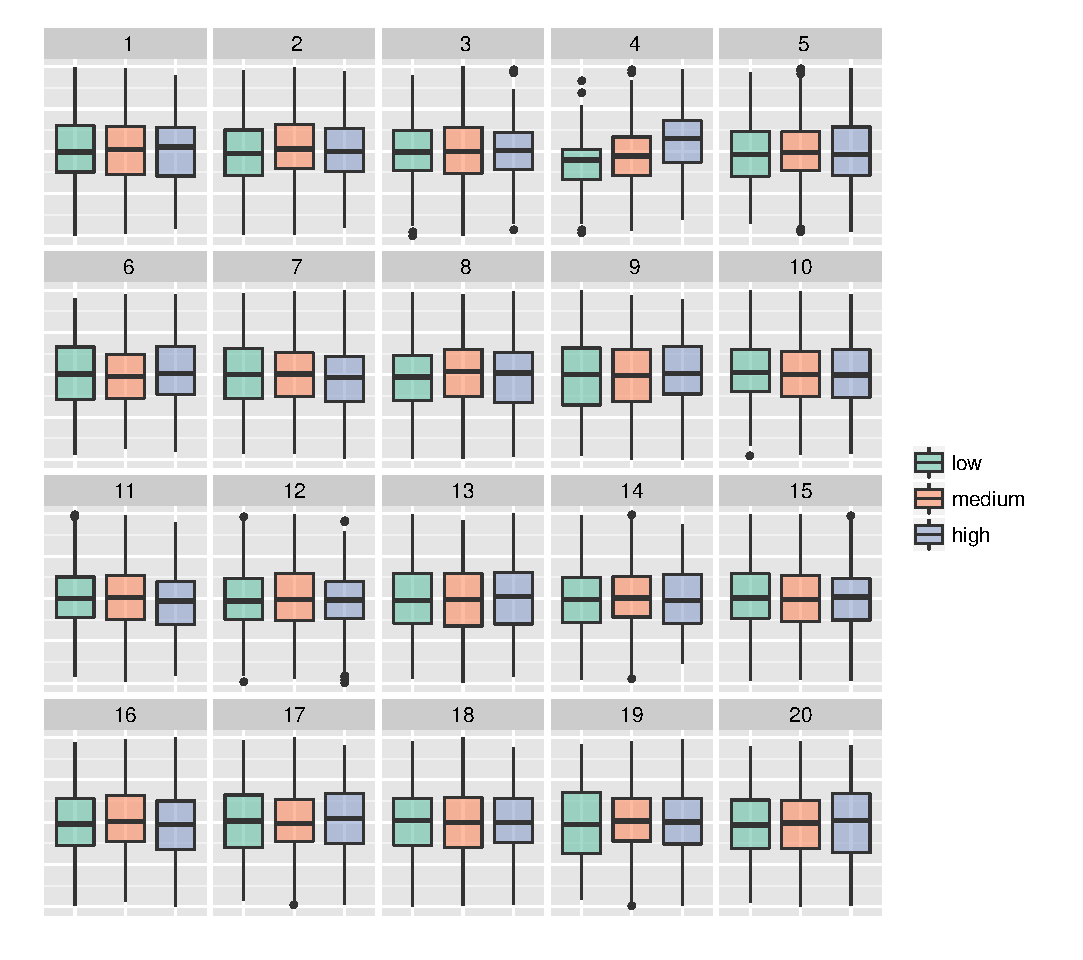
\includegraphics[width=\textwidth]{autism_sicdegp_level1_lineup5.pdf}
	\caption{\label{fig:boxplot-ordered} Lineup testing for the significance of social skills (low, medium, or high) for a longitudinal model investigating investigating the development of social skills from childhood to adolescence for children diagnosed with autism spectrum disorder. Here the level-1 residuals are used to see if the variable accounts for any additional residual variability. Which is the real plot?}
\end{figure}

\todo[inline]{I also included the unordered boxplots so we could look at the difference}

\begin{figure}
	\centering
	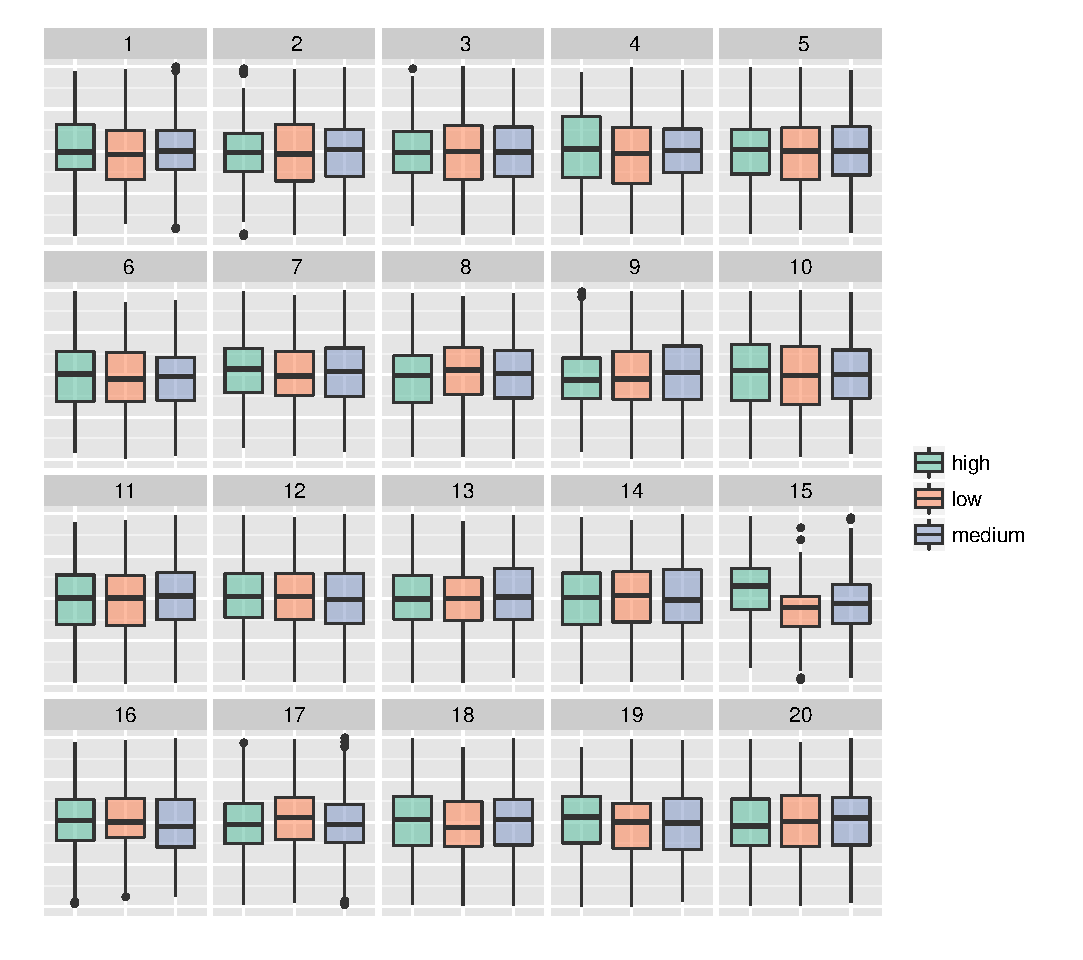
\includegraphics[width=\textwidth]{autism_sicdegp_level1_lineup4.pdf}
	\caption{\label{fig:boxplot-unordered} Lineup testing for the significance of social skills (low, medium, or high) for a longitudinal model investigating investigating the development of social skills from childhood to adolescence for children diagnosed with autism spectrum disorder. Here the level-1 residuals are used to see if the variable accounts for any additional residual variability. Which is the real plot?}
\end{figure}

%To illustrate the use of visual tests for fixed effects...\todo{Choose a data set!}


\paragraph{Random effects.} Tests of the random part of a hierarchical model focus on two questions: (1) whether a marginal random effect improves the model and (2) whether allowing the random effects to be correlated improves the model. Different plots must be used to answer each question. To answer the first question, we suggest plots comparing the response and the explanatory variable of interest using appropriate (often linear) smoothers for each group. Scatterplots comparing the predicted random effects can be used to answer the second question.

\hh{The lineup in figure~\ref{fig:fanned} is chosen to test the relationship between scores from the General Certificate of Secondary Education exam (GCSEE) and the  standardized London Reading Test (LRT).  Each of the lines summarizes the relationship between GCSEE and LRT scores for one of 65  inner-London schools (see section~\ref{data:GCSE} for additional details).}
\hh{The question of interest is whether random slopes for LRT scores are required to  represent the relationship between GCSEE and LRT scores ($H_1$). Correspondingly, null plots  are  created by simulating GCSE exam scores from a random intercept model,} 
\al{and overlaying linear smoothers for each school.}
%
%Revisiting Figure~\ref{fig:fanned} we see an example of testing for the inclusion of a random effect. Recall that the initial model was a random intercept model using a student's score on the standardized London Reading Test to describe their age 16 score on the General Certificate of Secondary Education examination.
 %To construct this figure we used the parametric bootstrap to generate simulated GCSE exam scores, fit separate regression models to the simulated responses, and then plotted the fitted model for each school. 
 If the model is appropriate, then these smoothers should resemble the observed data. In this example, we find that the true plot (panel $\sqrt{144} + 1$) is indentifiable as the variance of GCSEE scores is larger for higher scores on the standardized LRT than in the null plots; thus, we find evidence supporting the inclusion of a random slope for standardized LRT. This conclusion agrees with the results of the likelihood ratio test, and did not require the use of an asymptotic distribution to calculate the $p$-value.

Having considered the value of a random slope in the model, we next consider whether the model needs to allow the random slope and intercept to be correlated ($H_1$). While this is an example of a standard likelihood ratio test problem, as a correlation of 0 is not on the boundary of the parameter space, a using a lineup keeps tests of the random effects in a unified framework. The lineup in Figure~\ref{fig:ranef-corr} shows scatterplots of the predicted random effects with a linear smoother. The null plots are created by simulation from the model that does not allow for correlation between the random effects, and the true plot is created using the predicted random effects from a model allowing for correlation between the random effects. If the correlation between the random effects is not necessary, then the true plot will display little correlation and be indistinguishable from the null plots. In Figure~\ref{fig:ranef-corr} the true plot (panel $\sqrt{70 + 11}$) is easily identified, providing evidence supporting the inclusion of the additional parameter.

\begin{figure}
	\centering
	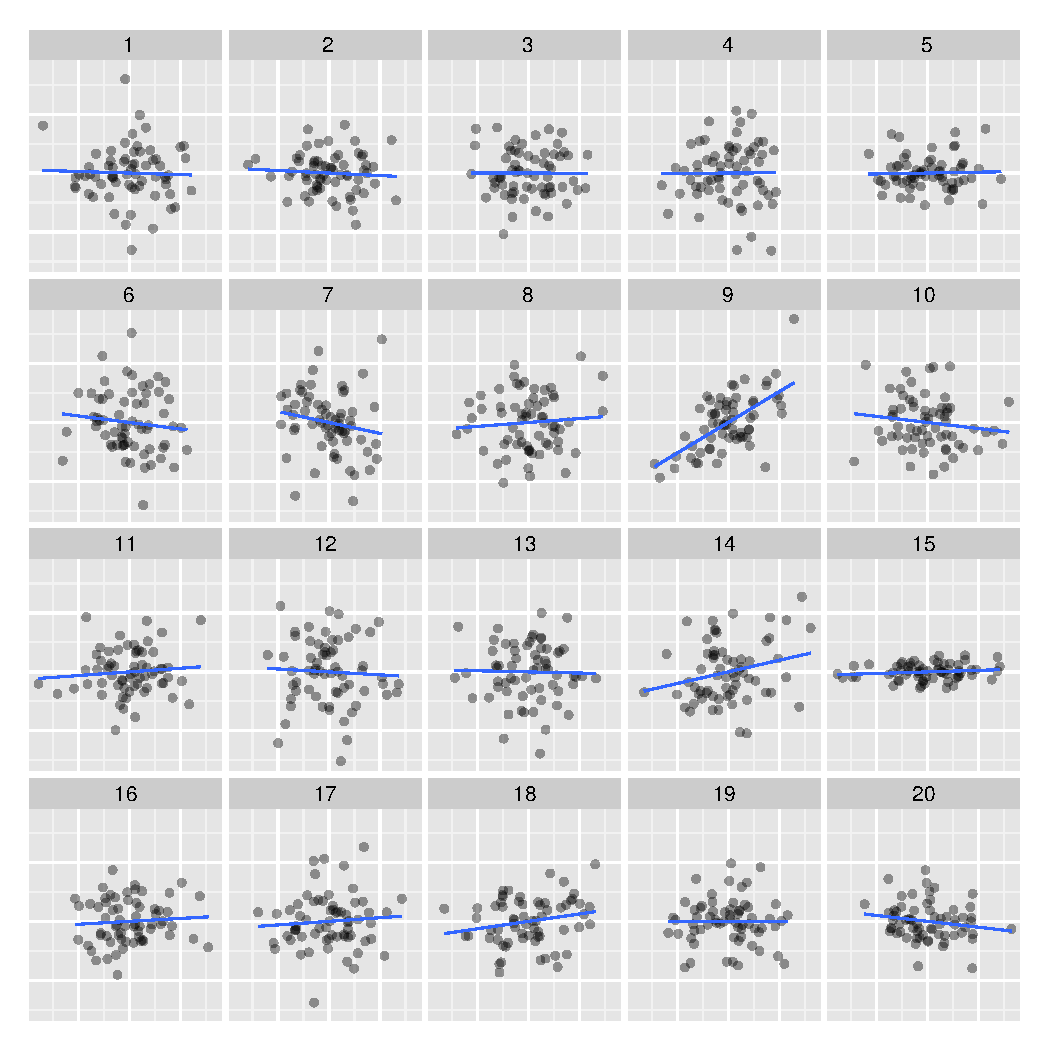
\includegraphics[width=\textwidth]{normexam_corr_lineup9.pdf}
	\caption{\label{fig:ranef-corr} Lineup testing the need to allow for correlation between the two random effects. These 20 plots compare the predicted random intercept and slope for the model fit to the Exam data. Which is the real plot? Note that this is the type of plot that \cite{Morrell:2000ve} discussed. If there were a higher degree of shrinkage in the random effects we would start to see more false lines in these plots, but as it is, if you remove the smoother and use $\alpha$-blending a line/curve is visible consisting of the random effects of children with only one observation.}
\end{figure}

\paragraph{Comparing non-nested models.}
If two non-nested models are being considered, visual inference can be used to investigate the goodness-of-fit of each model (see Section~\ref{sec:checking} for further discussion). If inadequacies are discovered in one model but not in the other, then this support the use of the properly specified model. This approach is similar in concept to comparing the AIC from each model; however, by focusing on an investigation of how the true data depart from the assumptions made by the model we can see why one may be preferred.


%------------------------------------------------------------------------------------
\subsection{Model checking}\label{sec:checking}
%------------------------------------------------------------------------------------

\subsubsection{Conventional practices}
%------------------------------------------------------------------------------------

\paragraph{Residual scatterplots/boxplots.} 
One of the most common diagnostic plots is a scatterplot or boxplot of the residuals (either level-1 or -2) against the fitted values or an explanatory variable. Such plots are often used to check linearity of the variables included in the model and homoscedasticity of the level-1 residuals. Patterns in these plots indicate departures from the model assumptions, however, we have found that patterns seem to be detectable in properly specified models more often than in the classical linear model. This problem is more commonly seen in scatterplots. 

\paragraph{Testing homoscedasticity across groups.}
Residual scatterplots are often used to check the assumption of homoscedastic level-1 residuals, but such plots do no account for the potential differences in variability across groups. Side-by-side boxplots of the level-1 residuals can be used to visualize this assumption; however, unbalanced group sizes can cause artificial structure in such plots. This can be seen by considering the sampling distribution of the level-1 residual variance, which has variance $\var \left( s_i^2 \right) = \left(2 \left( \sigma_i^2 \right)^2 \right) \big/ (n_i - p_i)$ which depends on the group size. Alternatively, \cite{Raudenbush:2002} propose using a standardized measure of dispersion given by
%
\begin{equation}\label{eq:d}
	d_i = \frac{\log\left( s_i^2 \right) - \left[ \sum_i (n_i - r_i) \log\left( s_i^2 \right) / \sum_i  (n_i - r_i) \right]}{\left(2 / (n_i - r_i)\right)^{1/2}}
\end{equation}
%
where $s_i^2$ is the residual variance within each group and $r_i = \mathrm{rank}(\bm{X}_i)$. The test statistic is then
%
\begin{equation}
	H = \sum_{i=1}^{m^*} d_i^2
\end{equation}
%
which has an approximate $\chi^2_{m^*-1}$ reference distribution when the data are normal and the group sizes are ``large enough''. Here we use $m^*$ because ``small'' groups may be excluded from the calculation as small group sizes provide less reliable information about the residual variance, but this is a subjective choice. If the distributional assumptions are violated or we do not have large enough group sizes, then the approximation to the $\chi^2$ distribution breaks down.


\paragraph{Quantile-Quantile plots.}
Quantile-Quantile (Q-Q) plots are often used as an informal check of the distributional assumptions made on the level-1 and -2 residuals; however, an interrelationship between the residual quantities exists in hierarchical linear models that can render such an assessment inappropriate. Additionally, strong assumptions are required for the empirical distributions of the residuals in the hierarchical linear model to converge in probability to their true distributions \citep[Theorem 3.2 and Lemma 3.1]{Jiang:1998vt}. If these assumptions are not satisfied, then the empirical distribution of the residuals may not resemble the hypothesized distribution under a properly specified model. Consequently, Q-Q plots will often lead to erroneous conclusions about the distributional assumptions.


\subsubsection{Proposals for visual inference}
%------------------------------------------------------------------------------------



\todo[inline]{The below sections are messed up because I am restructuring again}

%------------------------------------------------------------------------------------
\section{Visual inference for hierarchical linear models}
%------------------------------------------------------------------------------------

In this section we discuss how visual inference can be implemented to conduct common tests for hierarchical linear models and to avoid misinterpreting residual plots. 


\subsection{Model selection}
%------------------------------------------------------------------------------------





%\begin{figure}
%	\centering
%	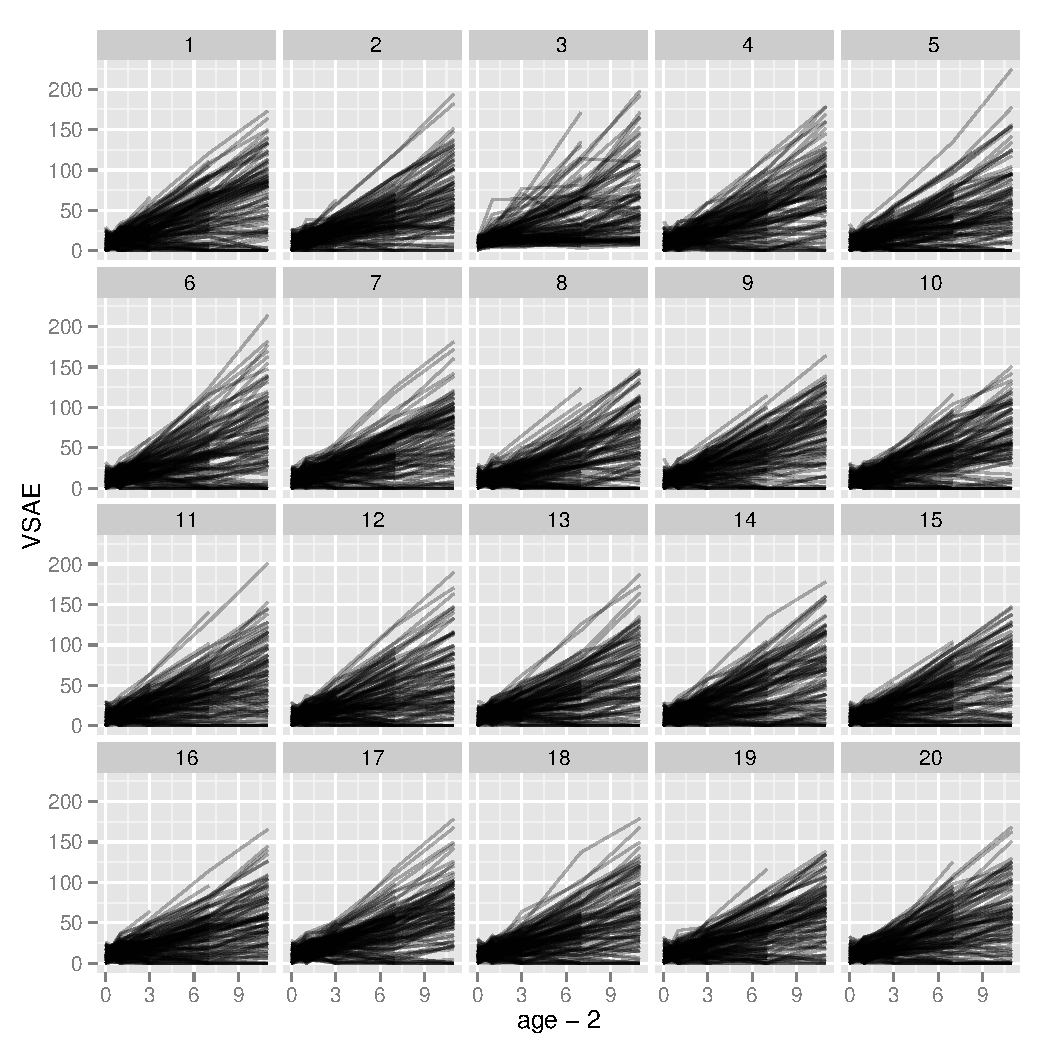
\includegraphics[width=\textwidth]{ranef1_lineup3.pdf}
%	\caption{\label{fig:lineup-ranef1} Lineup testing whether the random slope for $(\text{age} - 2)$ is sufficient, or if additional random effects are needed. These 20 plots display a child's VSAE trajectory. Which is the real plot?}
%\end{figure}
%
%\begin{figure}
%	\centering
%	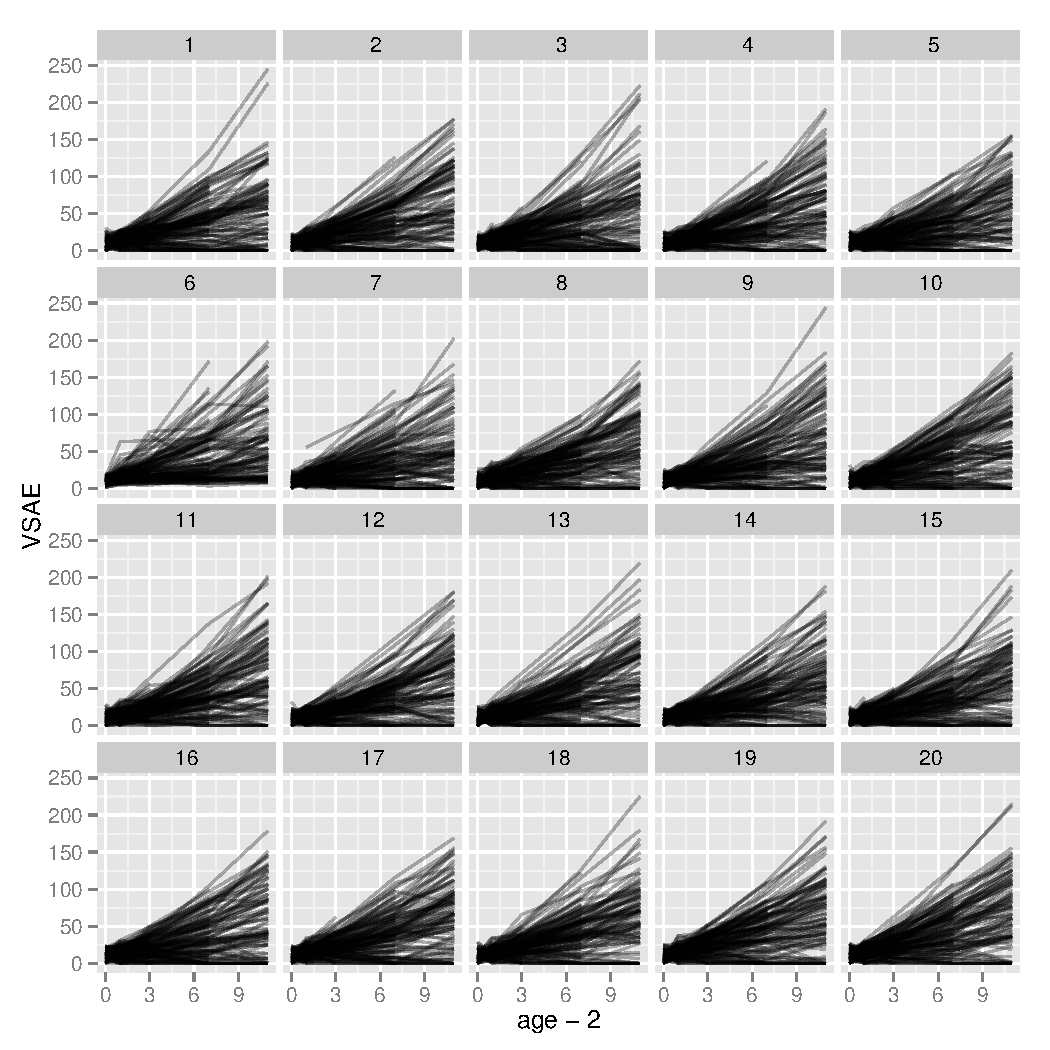
\includegraphics[width=\textwidth]{ranef2_lineup6.pdf}
%	\caption{\label{fig:lineup-ranef2} After adding a random effect for $(\text{age} - 2)^2$ we can construct the same lineup to see if we have a sufficient representation of the relationship between VSAE and age. These 20 plots display a child's VSAE trajectory. Which is the real plot?}
%\end{figure}


\begin{figure}
	\centering
	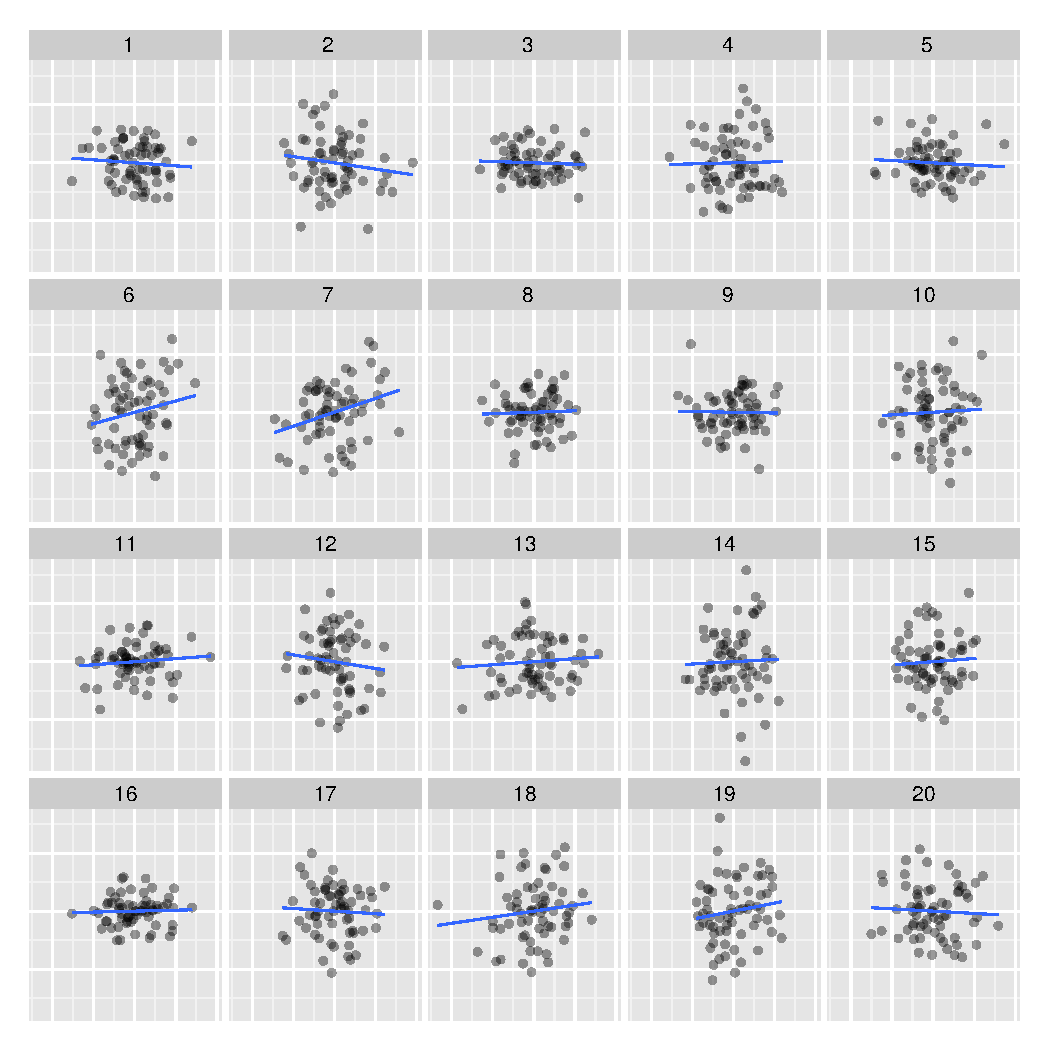
\includegraphics[width=\textwidth]{normexam_uncorr_lineup13.pdf}
	\caption{\label{fig:ranef-uncorr}  Lineup testing the need to allow for correlation between the two random effects. These 20 plots compare the predicted random intercept and slope for the model fit to the Exam data. Which is the real plot?}
\end{figure}

\begin{figure}
	\centering
	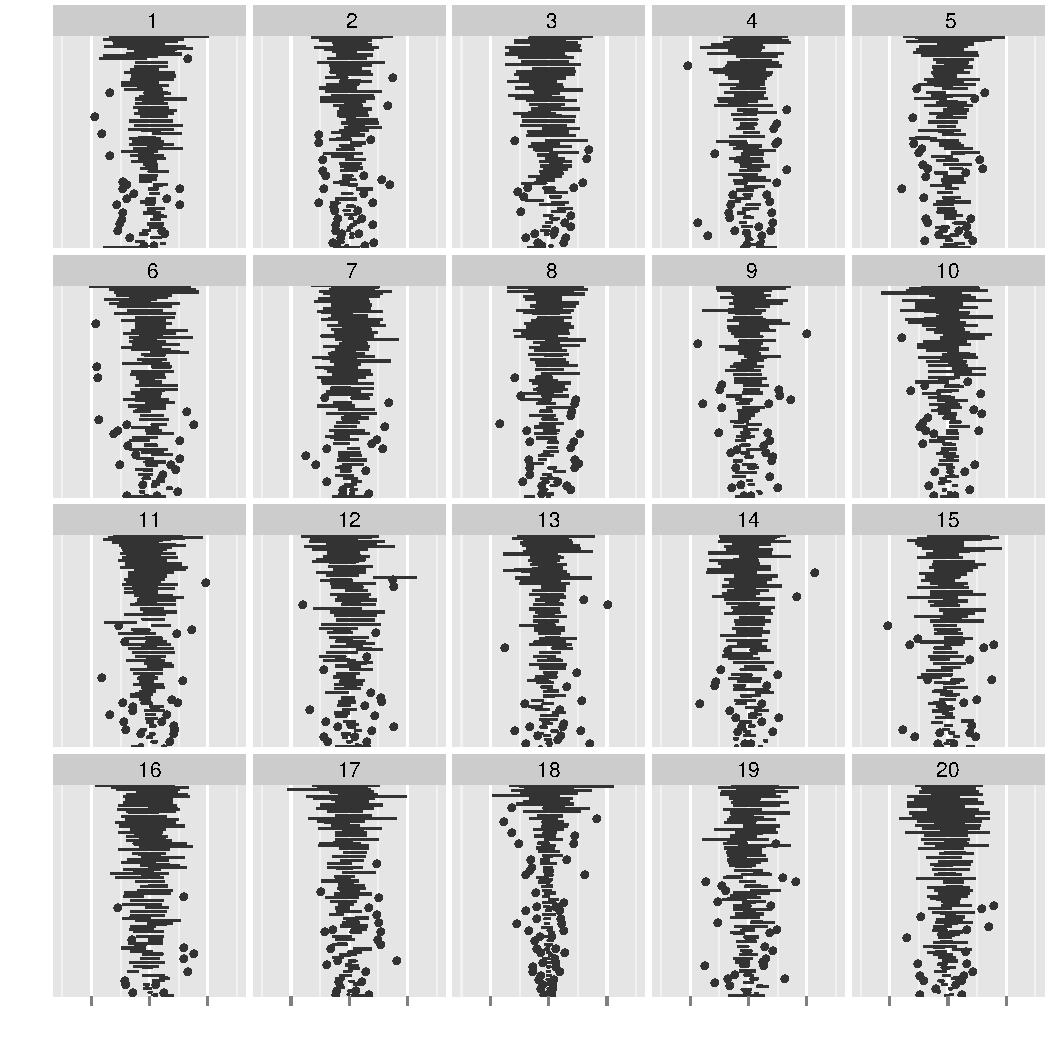
\includegraphics[width=\textwidth]{ahd_badcyclone5.pdf}
	\caption{\label{fig:badcyclone} Lineup of 20 boxplots (ordered by IQR) of level-1 residuals used to test the assumption of homogeneous level-1 residual variance.  Which is the real plot?}
\end{figure}

\begin{figure}
	\centering
	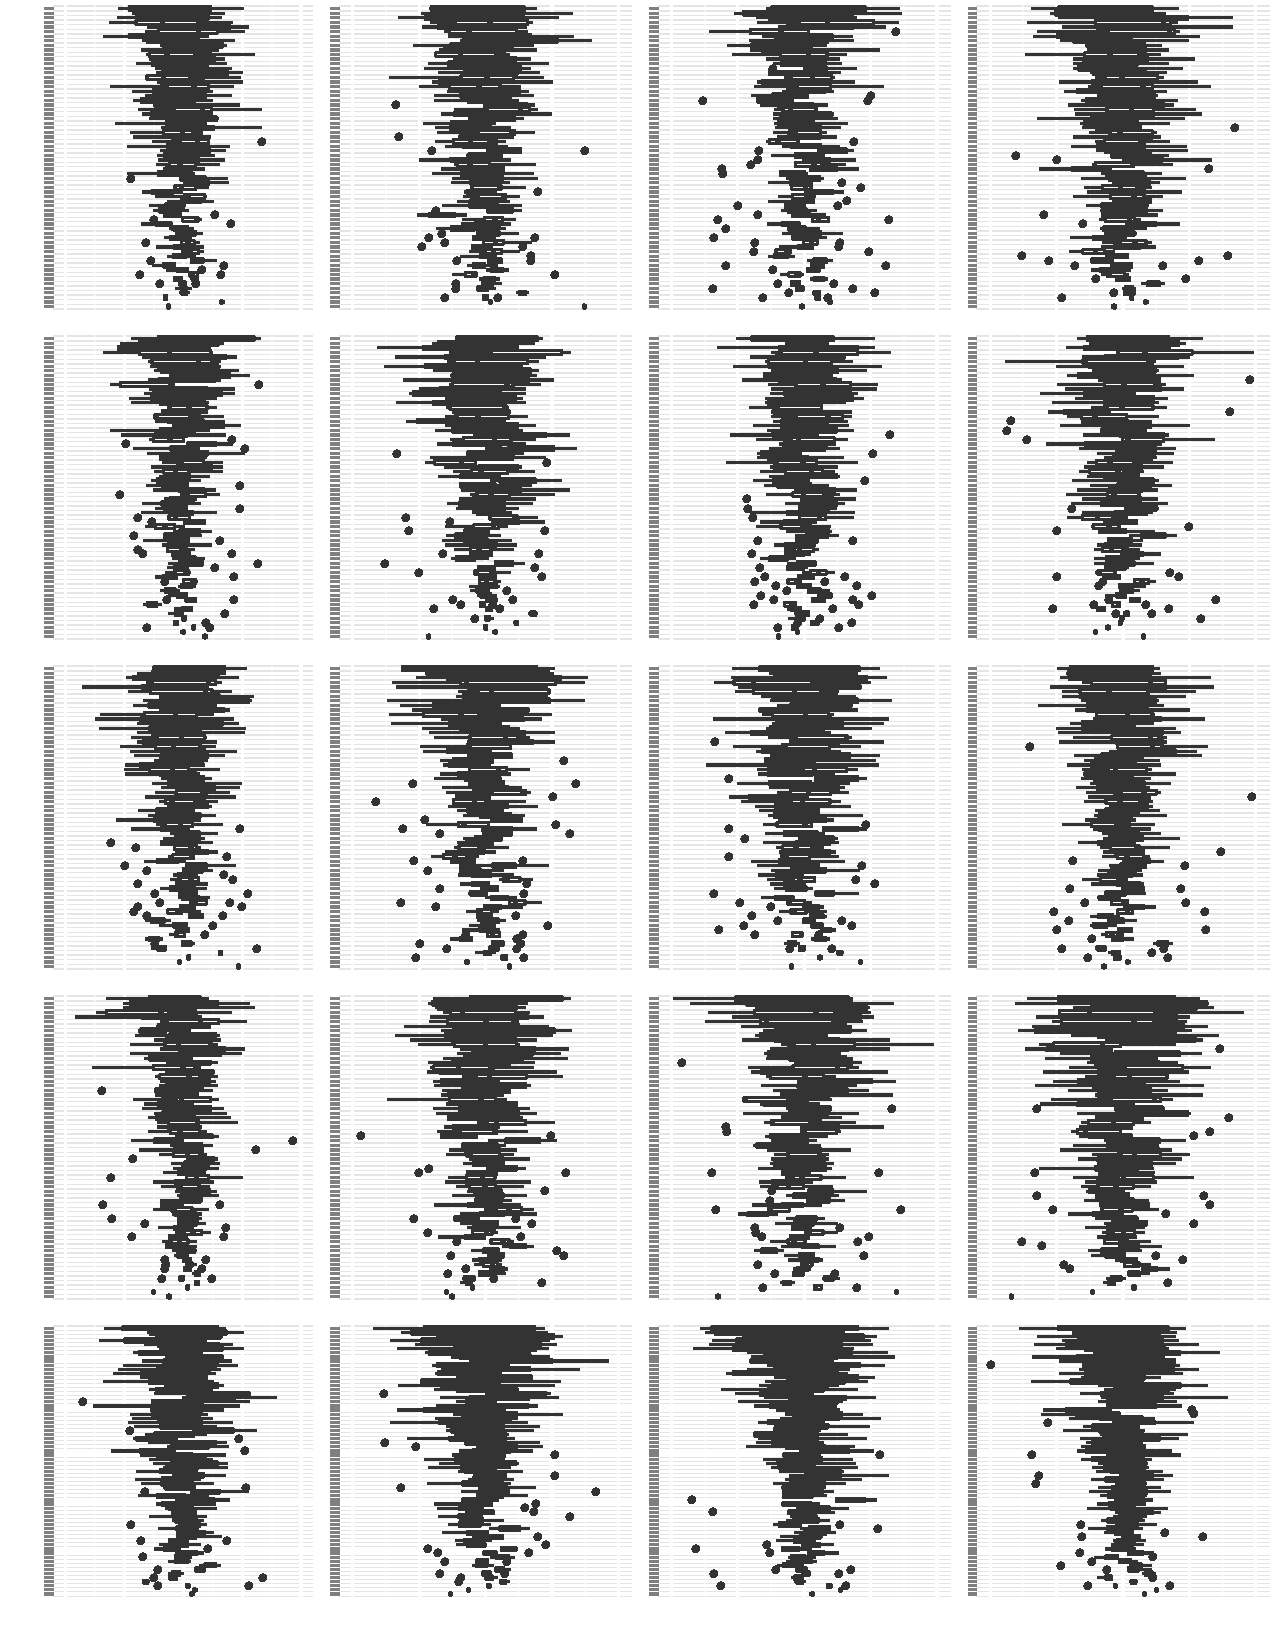
\includegraphics[width=\textwidth]{ahd_goodcyclone13.pdf}
	\caption{\label{fig:goodcyclone} Lineup of 20 boxplots (ordered by IQR) of level-1 residuals used to test the assumption of homogeneous level-1 residual variance.  Which is the real plot?}
\end{figure}

\begin{figure}
	\centering
	\includegraphics[width=\textwidth]{normexam_constvar_lineup5.pdf}
	\caption{\label{fig:constvar1} Lineup of 20 scatterplots of level-1 residuals against (standardized LRT)$^3$ used to test the assumption of homogeneous level-1 residual variance.  Which is the real plot?}
\end{figure}


\begin{figure}
	\centering
	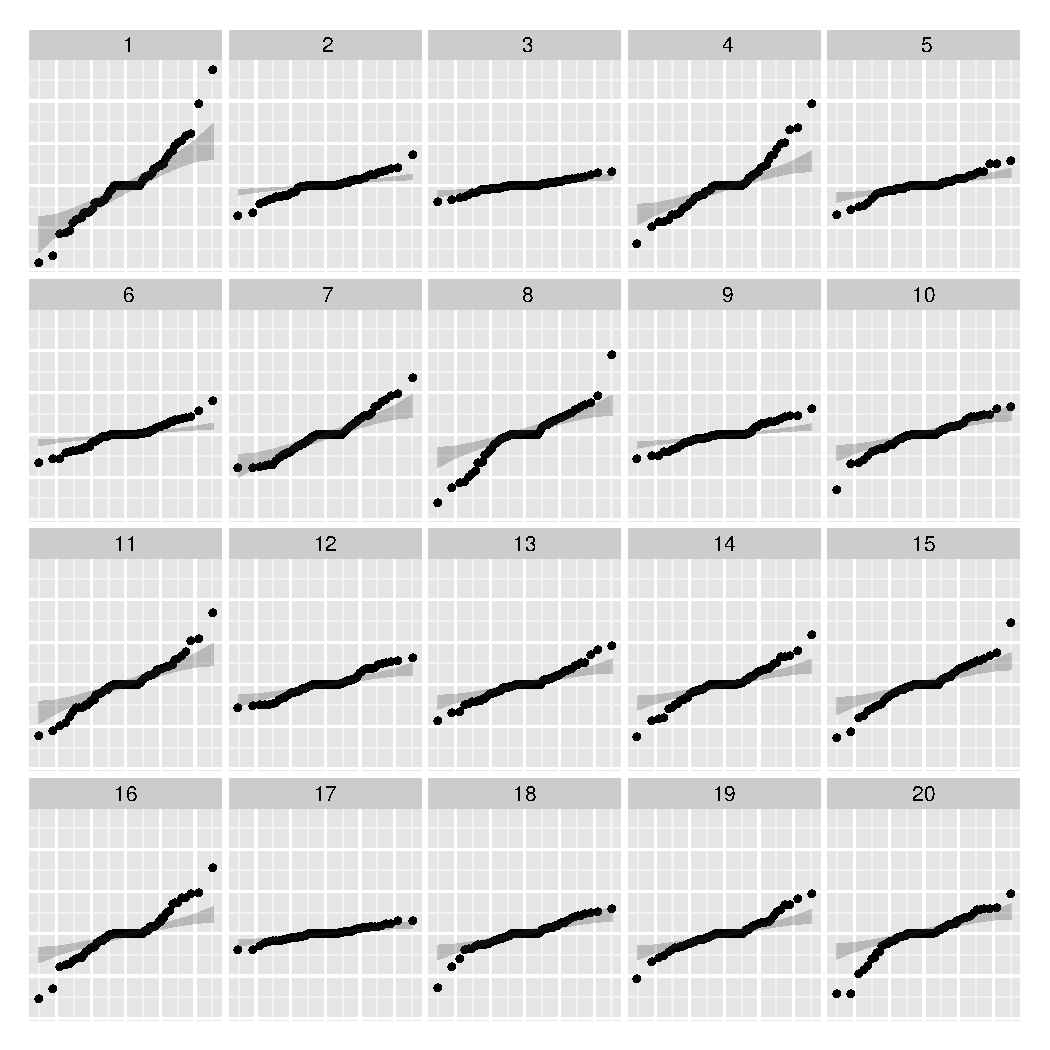
\includegraphics[width=\textwidth]{qqplot_normranef_slope_lineup11.pdf}
	\caption{\label{fig:qqlineup-norm} Lineup of 20 normal Q-Q plots for the predicted random slope.  Which is the real plot?}
\end{figure}

\begin{figure}
	\centering
	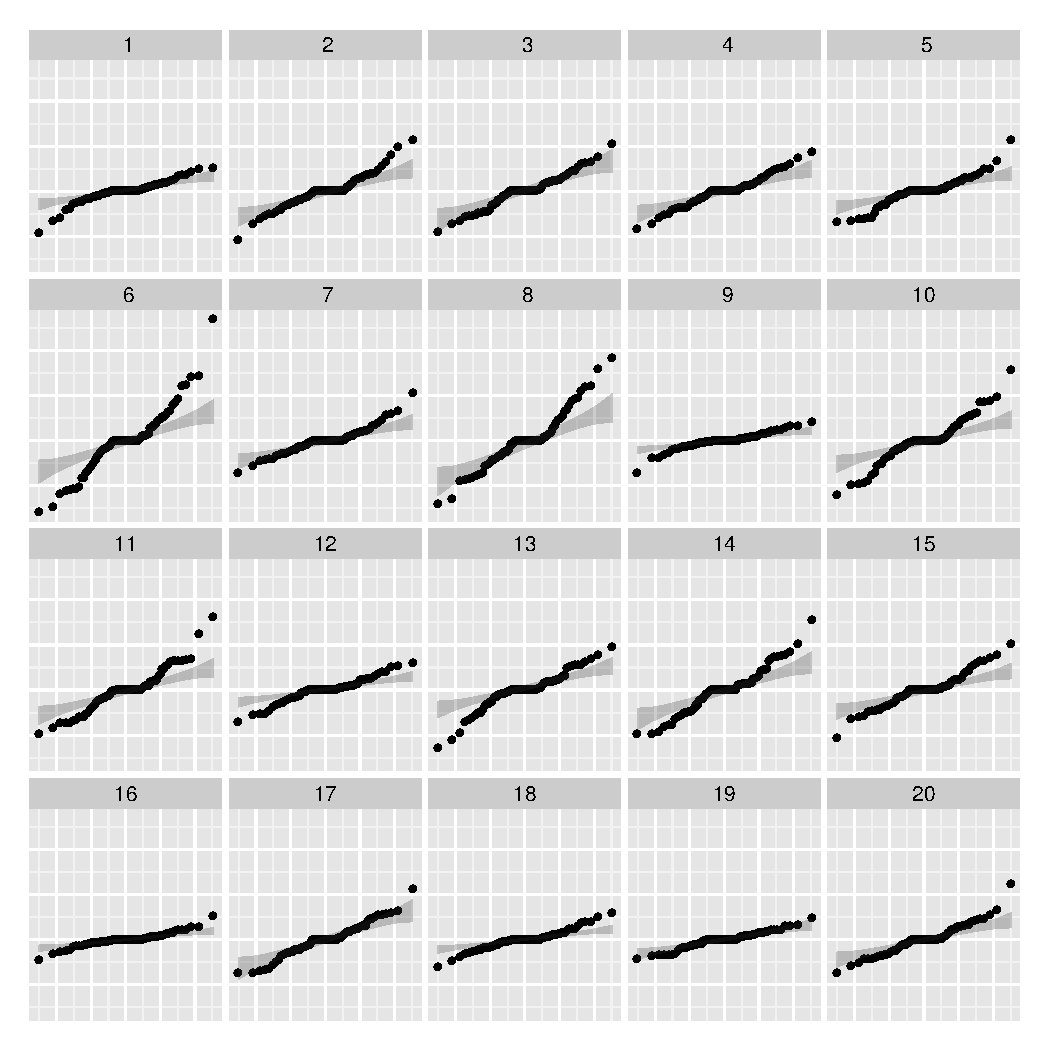
\includegraphics[width=\textwidth]{qqplot_tranef_slope_lineup6.pdf}
	\caption{\label{fig:qqlineup-t} Lineup of 20 normal Q-Q plots for the predicted random slope.  Which is the real plot?}
\end{figure}

\subsection{Model checking}
%------------------------------------------------------------------------------------

Include:
\begin{itemize}
\item Checks for level-1 and -2 heteroscedasticity -- cyclone plots, residuals vs. predictors
\item Linearity

\end{itemize}


%\todo[inline]{Below is a list of some initial ideas.}
%%------------------------------------------------------------------------------------
%\section{}
%%------------------------------------------------------------------------------------
%Applications of hierarchical models:
%\begin{itemize}
%\item Education -- students nested in classes nested in schools
%\item Interviewer research -- respondents nested in interviewer (Hox 1994)
%\end{itemize}
%
%Situations to consider:
%\begin{itemize}
%\item Residual analysis
%	\begin{itemize}
%	\item Unbalanced sample sizes introduces structure
%	\item Using raw rather than standardized residuals can introduce structure
%	\item This could help avoid using theoretical cutoffs for statistics used in the detection of outliers and influential points. \cite{Longford:2001wy} discusses numeric simulation-based diagnostics for outlier and makes some good points about how the theoretical distributions of these statistics are: (1) hard to calculate theoretically in many situations; (2) are based on a unit being randomly selected, as opposed to selected after an inspection of the data.
%	\end{itemize}
%
%\item Comparison of random effects -- \cite{Morrell:2000ve} discuss lines in plots of random effects appear when there are groups with a large amount of pooling (shrinkage)
%
%\item Exploratory modeling
%	\begin{itemize}
%	\item Considering a variable for inclusion in the model as a fixed effect
%	\item The need for/utility of additional random effects
%	
%	\end{itemize}
%
%
%\end{itemize}


%------------------------------------------------------------------------------------
\section{Investigating Q-Q plots visually}
%------------------------------------------------------------------------------------

We are testing three different versions of a Q-Q plot %\citep{Wilk:1968}, 
see figure~\ref{qqplots}. From left to right, a standard Q-Q plot, a Q-Q plot with an added confidence region based on a simulation envelope of the theoretical distribution, and a rotated Q-Q plot of the same data are shown. 

\begin{figure}
%<<qqplots, fig.width=2.75, fig.height=2.75, out.width='0.3\\textwidth', echo=FALSE, include=FALSE>>=
%dframe <- read.csv("data/data-1-1-1-20-2-14-5.csv")
%library(ggplot2)
%dframe$.sample <- "Control"
%ctrl_lineup(subset(dframe, .sample_outer==5))
%dframe$.sample <- "Standard"
%std_lineup(subset(dframe, .sample_outer==5))
%dframe$.sample <- "Rotated"
%rot_lineup(subset(dframe, .sample_outer==5))
%@
\centering
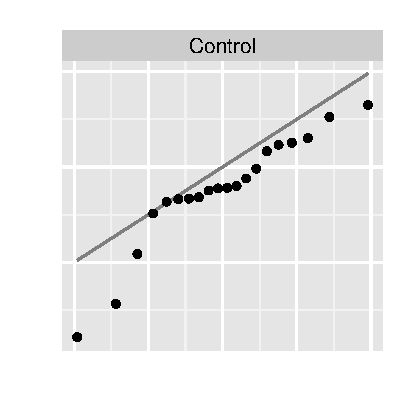
\includegraphics[width=0.3\textwidth]{qqplots1}
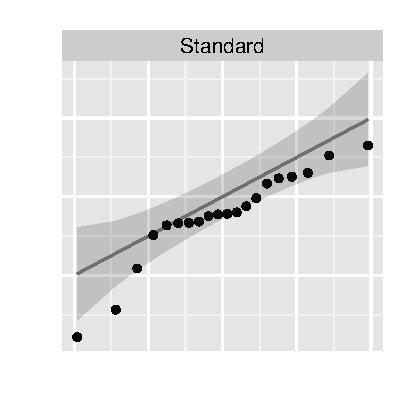
\includegraphics[width=0.3\textwidth]{qqplots2}
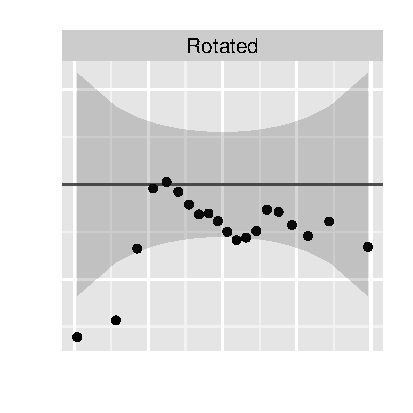
\includegraphics[width=0.3\textwidth]{qqplots3}
\caption{ \label{qqplots} Three versions of Q-Q plots: control, standard, and rotated.}
\end{figure}

%------------------------------------------------------------------------------------
\section{Discussion and conclusions}
%------------------------------------------------------------------------------------


%------------------------------------------------------------------------------------
\section{Acknowledgment}
%------------------------------------------------------------------------------------
This work was funded in part by National Science Foundation grant DMS 1007697.

%------------------------------------------------------------------------------------
\section{Appendix: Data sets}
%------------------------------------------------------------------------------------
\subsection{General Certificate of Secondary Education}\label{data:GCSE}

We make use of a subset of examination results of 4,065 students nested within 65 inner-London schools discussed by \cite{Goldstein:1993wm}. The original analysis explored school effectiveness as defined by students' performance on the General Certificate of Secondary Education (GCSE) scores in both mathematics and English. This exam is taken the end of at the end of compulsory education, typically when students are 16 years old.  To adjust for a student's ability when they began secondary education, the students' scores on the standardized London Reading Test (LRT) and verbal reasoning group (bottom 25\%, middle 50\%, or top 25\%) at age 11. Additional information contained in the data set includes student gender, school gender, and the average LRT intake score for each school.

%------------------------------------------------------------------------------------

\subsection{The autism data}\label{data:autism}
%------------------------------------------------------------------------------------

Autism is a developmental disorder typically characterized by impaired communication and social skills, but there is relatively little consensus on how these abilities or disabilities change over time \citep{Anderson:2007cl, Anderson:2009in}. In an effort to better understand changes in verbal and social abilities from childhood to adolescence \cite{Anderson:2007cl, Anderson:2009in} carried out a prospective longitudinal study following following 214 children between the ages of 2 and 13 who had been diagnosed with either autism spectrum disorder or non-spectrum developmental delays at age 2. 
The Vineland Adaptive Behavior Interview survey was used to assess each child's interpersonal relationships, play time activities, and coping skills. This survey is completed by the parents. From the survey the Vineland Socialization Age Equivalent (VSAE) was computed as overall measure of a child's social skills. Additionally, expressive language development at age 2 was assessed using the Sequenced Inventory of Communication Development (SICD) and the children were classified into three groups (high, medium, or low). Assessments were made on the children ages 2, 3, 5, 9, and 13, however, not all children were assessed at each age. Additional information collected on each child includes: gender, race (white or non-white), and initial diagnosis at age 2 (autism, pervasive development disorder (pdd), or non-spectrum). We restrict attention to models concerned with the changes in social skills for subjects diagnosed with autism spectrum disorder having complete data. This results in a reduced data set of 155 children. For more detailed analyses we refer the reader to \cite{Anderson:2007cl, Anderson:2009in}.


%------------------------------------------------------------------------------------
%------------------------------------------------------------------------------------

\bibliographystyle{apalike}
\bibliography{hlmviz_bib}

\end{document}